\chapter{The Helly and Strong Helly numbers fo graphs $B_k$-EPG and $B_k$-VPG}
\label{cap:iv}

\begin{flushright}
\begin{minipage}[t][0cm][b]{0.47\textwidth}
\emph{
%A Matemática é o alfabeto com o qual Deus escreveu o Universo.
Falta algo para completar esta demonstração, mas não tenho tempo.}
\end{minipage}

\rule[0cm]{7cm}{0.03cm}%{largura}{espessura}

Évariste Galois
\end{flushright}




O estudo de grafos EPG foi introduzido por  Golumbic, Lypshteyn e Stern (2009) e consiste dos grafos de intersecção de conjuntos de caminhos sobre uma grade ortogonal, cujas intersecções são tomadas considerando as arestas dos caminhos. Se as intersecções dos caminhos consideram os vértices e não as arestas, a classe de grafos resultante é chamada de grafos VPG. Tal classe foi introduzida em 2011 \cite{asinowski2011string} e \cite{asinowski2012}. Nesse capítulo estudaremos dois parâmetros em ambas classes de grafos EPG e VPG. Os parâmetros que serão estudados são nomeadamente o número de Helly e o número de Helly forte.

\section{Discussão Inicial}

Seja  $\cal {F}$ uma família de conjuntos de algum conjunto universal $U$, e $h$ um número inteiro tal que $h\geq 1$. Podemos dizer que $\cal{F}$ é $h$-{\it intersectante} quando todos  $h$ subconjuntos de $\cal {F}$ intersectam-se. Chamamos de {\it core} de $\cal {F}$ a intersecção de todos conjuntos de $\cal {F}$, e denotamos por $core(\cal F)$. 

A família $\cal{F}$ é $h$-{\it Helly} quando toda subfamília $h$-intersectante $\cal{F'}$ satisfaz $core(\cal{F'}) \neq \emptyset$, ver mais em \cite{duchet1978propriete}. Por outro lado, se para toda subfamília $\cal{F'}$ de $\cal{F}$, existem $h$ subconjuntos cujo core é igual ao core de  $\cal {F'}$, então $\cal {F}$ é dito ser  $h$-{\it Helly} {\it forte}. Claramente, se $\cal {F}$ é $h$-Helly então ele também é $h'$-Helly, para $h' \geq h$. Similarmente, se ${\cal F}$ é $h$-Helly forte então ele também é $h'$-Helly forte, para $h' \geq h$. 

Finalmente, o   {\it número de Helly} da família  $\cal{F}$ é o menor inteiro $h$, tal que $\cal{F}$ é  $h$-Helly. Similarmente, o {\it número de Helly forte} de  $\cal{F}$ é o menor $h$, para o qual  $\cal{F}$ é  $h$-Helly forte. Também segue que o número de Helly forte de $\cal{F}$ é no mínimo igual ao seu número de Helly.


Uma  {\it classe} $\cal {C}$ de famílias $\cal {F}$  de subconjuntos de algum conjunto universal $U$ é uma  subcoleção das famílias $\cal {F}$ de $U$. Dizemos que  $\cal C$ é uma {\it classe hereditária}, quando ela é fechada sob inclusão, i.e. se um grafo $G$ pertence a uma classe $C$ então todo subgrafo induzido de $G$ também pertence a $C$. O {\it número de Helly}  de uma classe  $\cal{C}$ de famílias $\cal{F}$ de subconjuntos é o maior número de Helly entre todas as famílias de $\cal {F}$. Similarmente, o {\it número de Helly forte} de uma classe  $\cal {C}$ é o maior número de Helly forte das famílias de $\cal {C}$.

Se $\cal F$ é uma família de subconjuntos e $\cal C$ uma classe de famílias, denotamos por $H(\cal F)$ e por 
$H(\cal C)$,  o número de  Helly de $\cal F$ e $\cal C$, respectivamente, enquanto  $sH({\cal F})$ e $sH({\cal C})$  representam os números de  Helly forte de $\cal F$ e $\cal C$.


Nesse capítulo, nos preocupamos com famílias de subconjuntos $\cal{F}$ de caminhos de arestas e vértices em uma grade. No primeiro contexto, consideramos que cada caminho $P_i$  consiste de uma sequência de arestas consecutivas na grade ortogonal, que forma o caminho, e chamaremos essas de   {\it representações EPG}. Dessa forma, segue que dois caminhos intersectam-se se e somente se eles contém no mínimo uma aresta da grade em comum. Aos grafos que  correspondem às representações EPG denotaremos por {\it grafos EPG}. 
No segundo contexto, um caminho é visto como uma sequência de vértices consecutivos, e dois caminhos intersectam-se se eles contém um vértice comum. Analogamente aos anteriores esses são chamados de {\it representações VPG} e {\it grafos VPG}. 

Cada aresta possui uma direção associada na grade, a qual pode ser horizontal ou vertical. Uma  {\it dobra} no caminho é um par de arestas consecutivas que possuem direções distintas.  Um {\it segmento} de um caminho é uma sequência de arestas consecutivas do caminho, sem dobras. Dizemos que o caminho $P_i$ é um  $B_k$-{\it path} se ele contém $k$ dobras. Dizemos que $\cal {F}$ é uma família de $B_k$-caminhos, ou simplesmente  uma $B_k$-família, se cada caminho de $\cal {F}$ contém no máximo $k$ dobras. 

 Nesse capítulo, resolvemos completamente o problema de determinar ambos o número de Helly e o número de Helly forte, para ambos contextos de grafos $B_k$-EPG e $B_k$-VPG. Determinamos o número de Helly em grafos $B_k$-EPG e $B_k$-VPG, para cada valor de $k$.

Para grafos EPG, o número de Helly de $B_0$-families é bem conhecido e é igual a 2, uma vez que  grafos $B_0$-EPG coincidem com grafos de intervalo. Também é simples concluir que o número de Helly forte dos grafos $B_0$-EPG é também igual a 2. Para $k = 1$,   provamos que ambos o número de Helly e número de Helly forte da classe de $B_1$-families são iguais a 3. Para a classe de  $B_2$-families, provamos que esses dois parâmetros são iguais a 4. Além disso o número de Helly e número de Helly forte para $B_3$-families é igual a 8, e finalmente esses parâmetros são ilimitados para  $k \geq 4$. 
Quanto aos grafos VPG, é simples concluir que o número de Helly de grafos $B_0$-VPG é igual a 2, e provamos que grafos $B_1$-VPG possuem número de Helly  4, grafos $B_2$-VPG possuem número de Helly  6, grafos $B_3$-VPG possuem número de Helly 12, enquanto o número de Helly para grafos $B_4$-VPG novamente é ilimitado.

Finalmente, o número de Helly forte é igual ao número de Helly nos grafos  $B_k$-EPG, para cada $k$. O mesmo vale para grafos $B_k$-VPG.

Com relação aos resultados existentes, 
Golumbic, Lipshteyn  e Stern \cite{golumbic2009} já tem mostrado que o número de Helly forte para grafos $B_1$-EPG é igual a 3, e para grafos $B_1$-VPG é igual a  4. Empregando técnicas de prova diferentes das utilizadas neste trabalho. Veja  \cite{golumbic2019edge}, Teorema 11.13, abaixo:
\begin{theorem}\label{thm:golumbic2019edge}{\cite{golumbic2019edge}}
Seja $P$ uma coleção de caminhos de dobra simples sobre uma grade. Se cada 2 caminhos em  $P$ compartilham no mínimo uma aresta da grade, então $P$ possui número de Helly forte igual a 3. Caso contrário, $P$ possui número de Helly forte igual a 4. 
\end{theorem}
Nenhum outro resultado relacionado ao número de Helly forte, ou resultados relacionados ao número de Helly de grafos $B_k$-EPG foi notado ter sido reportado na literatura levantada. Quanto a outras classes, Golumbic e Jamison  tem determinado o número de Helly forte dos caminhos de intersecção de arestas sobre uma árvore em~\cite{golumbic1985}. Finalmente, Asinowski, Cohen, Golumbic, Limouzy, Lipshteyn e Stern tem reportado que o número de Helly forte de grafos $B_0$-VPG é igual a 2 \cite{asinowski2011string}.  
Alguns resultados relacionados estão listados a seguir. Decidir se um dado hipergrafo é  $k$-Helly pode ser feito em tempo polinomial para um  $k$ fixo,  empregando a caracterização proposta por Berge e Duchet \cite{bergeDuchet1975}. Para algum $k$ arbitrário, o problema é  \cal{co-NP}-completo \cite{dourado2009}. Para ver mais problemas correspondendo à propriedade $k$-Helly forte e exemplos sugerimos a leitura de~\cite{dourado2008strong,dourado2009}.

Este capítulo está organizado como listado a seguir. A seção~\ref{sec:preliminares4}, contém algumas proposições preliminares e notações adicionais utilizadas neste escrito. A seção~\ref{sec:Helly-number}  descreve os resultados para o número de Helly de grafos $B_k$-EPG, enquanto a seção~\ref{sec:helly-vpg} contém resultados desse parâmetro para grafos $B_k$-VPG. O número de Helly forte é considerado na seção~\ref{sec:helly-forte}. Considerações finais são efetuadas na seção~\ref{sec:finalRemarks4}.

\section{Preliminares}\label{sec:preliminares4}

O seguinte teorema caracteriza famílias de subconjuntos $h$-Helly.


\begin{theorem}\label{thm:BD}(\cite{bergeDuchet1975}):
Uma família $\cal{F}$ de subconjuntos do conjunto universal  $U$ é $h$-Helly se e somente se para todo subconjunto   $U' \subseteq U$, $|U'|= h+1$,  a subfamília  $\cal{F'}$ de $\cal{F}$,  formada pelos subconjuntos contendo no mínimo  $h$ dos $h+1$ elementos de $U'$, tem um core não vazio. 
\end{theorem}

O próximo teorema é central para os nossos resultados.

\begin{theorem}\label{thm:minimal}Seja ${\cal C}$ uma classe hereditária de famílias ${\cal F}$ de subconjuntos do conjunto universal $U$, cujo número de Helly $H({\cal C})$ é igual a $h$. Então, existe uma família ${\cal F'} \in {\cal C}$ com exatamente $h$ subconjuntos, satisfazendo as seguintes condições: 

Para cada subconjunto  $P_i \in \cal {F'}$, existe exatamente um elemento distinto $u_i \in U$, tal que \\
$$u_i \not \in P_i,$$ 
mas $u_i$ está contido em todos subconjuntos 
$$P_j \in {\cal F'} \setminus P_i.$$
\end{theorem}
 

Proof: 
Seja ${\cal C}$ uma classe de famílias  ${\cal F}$ de subconjuntos $P$, cada subconjunto formado pelos elementos  $u \in U$, tal que o número de Helly $H({\cal C})$  é igual a $h$. Então cada família   ${\cal F} \in {\cal C}$ satisfaz $H({\cal F}) \leq h$. Considere uma família ${\cal F'} \in {\cal C}$  cujo número de Helly é  exatamente $h$, e contendo exatamente $h$ subconjuntos. Essa família deve existir uma vez que  ${\cal C}$ é uma classe hereditária. Além disso $H({\cal F'}) = h$, $\cal F'$ é $h$-intersectante, e portanto $(h-1)$-intersectante. Ademais, ${\cal F'}$ não é $(h-1)$-Helly. Aplicando o   Teorema~\ref{thm:BD}, podemos concluir que existem   $h$ elementos $U' = \{u_1, \ldots, u_h\} \subset U$, tal que cada conjunto de ${\cal F'}$ contem no mínimo $h-1$ elementos de $U'$. Uma vez que $H({\cal F'}) > h-1$, $core({\cal F'}) = \emptyset$ e além disso não existe elemento comum entre os conjuntos de $\cal F'$. Em particular, uma vez que cada conjunto $P_i \in {\cal F'}$ contem no mínimo  $h-1$ elementos de $U'$, e $core(\cal F') = \emptyset$, podemos escolher   $h$ subconjuntos $P_i$, em que cada um deles deixa de possuir um elemento distinto  $u_i \in U'$. Então para cada subconjunto  $P_i \in \cal F$, existe algum elemento $u_i \not \in P_i$, mas $u_i \in P_j$, para todos $P_j \in \cal F'$, $j \neq i$. \qed

Seja $\cal{ F'}$ como descrito no teorema anterior. É simples concluir que ao remover qualquer subconjunto de $\cal {F'}$ este torna-se $(h-1)$-Helly.  Todavia podemos chamar $\cal {F'}$ de uma {\it família minimal não}-$(h-1)$-{\it Helly}. Além do mais, o elemento $u_i \not \in P_i$, contido em todos os subconjuntos $P_j \in {\cal{F'}} \setminus P_i$, exceto $P_i$, é o {\it $h$-não-representativo} de $P_i$.  

Empregaremos as famílias de subconjuntos minimais citadas anteriormente, aplicadas à $B_k$-caminhos em uma grade. Note que $B_k$-caminhos em uma grade formam uma classe hereditária.

\section{O Número de Helly de Grafos $B_k$-EPG}\label{sec:Helly-number}

Nessa seção determinaremos o número de Helly das classes de grafos $B_1$-EPG, $B_2$-EPG e $B_3$-EPG, e mostraremos que para os grafos $B_k$-EPG, $k \geq 4$, o número de Helly é ilimitado. Provaremos os seguintes resultados.

\begin{theorem}\label{thm:Helly-EPG}
O número de Helly de grafos $B_k$-EPG satisfaz:
\begin{enumerate}[nosep,label=\emph{(\roman*)}]
\item  $H(B_1$-EPG) = 3 
\item $H(B_2$-EPG)  = 4 
\item $H(B_3$-EPG)  = 8 
\item $H(B_k$-EPG) é ilimitado, para 
$k \geq 4$.
\end{enumerate}

\end{theorem}

A prova consiste em determinar limites inferiores e limites superiores justos, como mostrado nas próximas subseções.

\subsection{Limites Inferiores}

Primeiro, descreveremos limites inferiores para o parâmetro número de Helly, como função do número de dobras $k$.

\begin{lema}\label{claim:lower-Bk-EPG} 
Os seguintes são limites inferiores para os grafos  $B_k$-EPG.
\begin{enumerate}[nosep,label=\emph{(\roman*)}]
\item   $H(B_1$-$EPG) \geq 3$ 
\item $H(B_2$-$EPG) \geq 4$ 
\item $H(B_3$-$EPG) \geq 8$ 
\item $H(B_k$-$EPG )$ é ilimitado para  $k \geq 4$.
\end{enumerate}
\end{lema}

\proof:

Para cada valor de  $k$, exibiremos uma $B_k$-família de caminhos em arestas na grade, tendo o número de dobras requerido, e cujo número de Helly é no mínimo o valor correspondente declarado. Nos referimos ao par de coordenadas dos pontos da grade (arestas da grade), de forma a descrever os caminhos.

\begin{figure}[!h]
\begin{center}
% \begin{tikzpicture}[line cap=round,line join=round,>=triangle 45,x=3.7mm,y=3.7mm]
% \draw [color=cqcqcq,, xstep=0.37cm,ystep=0.37cm] (-7,-1.4) grid (22.16,6.8);
% \clip(-5.7,-2.5) rectangle (25,9.6);
% \draw (-5,-1.3) node[anchor=north west] {(a)};
% \draw (2.5,-1.3) node[anchor=north west] {(b)};
% \draw (14.5,-1.3) node[anchor=north west] {(c)};
% \draw [line width=2pt] (4,0)-- (4,2)-- (6,2)-- (6,0);
% \draw [line width=2pt] (3,2)-- (1,2)-- (1,0)-- (3,0);
% %\draw (-0.3,3.7) node[anchor=north west] {0};
% %\draw (-0.3,5.1) node[anchor=north west] {1};
% %\draw (-0.3,6.1) node[anchor=north west] {2};
% \draw [line width=2pt] (1,5)-- (3,5)-- (3,3)-- (1,3);
% \draw [line width=2pt] (4,5)-- (4,3)-- (6,3)-- (6,5);
% %\draw (8.7,0.7) node[anchor=north west] {0};
% %\draw (8.7,2.1) node[anchor=north west] {1};
% %\draw (8.7,3.1) node[anchor=north west] {2};
% %\draw (8.7,3.7) node[anchor=north west] {0};
% %\draw (8.7,5.1) node[anchor=north west] {1};
% %\draw (8.7,6.1) node[anchor=north west] {2};
% \draw [line width=2pt] (10,5)-- (12,5)-- (12,3)-- (10,3)-- (10,4);
% \draw [line width=2pt] (14,5)-- (13,5)-- (13,3)-- (15,3)-- (15,5);
% \draw [line width=2pt] (19,3)-- (19,5)-- (21,5)-- (21,3)-- (20,3);
% \draw [line width=2pt] (18,4)-- (18,5)-- (16,5)-- (16,3)-- (18,3);
% \draw [line width=2pt] (10,1)-- (10,2)-- (12,2)-- (12,0)-- (10,0);
% \draw [line width=2pt] (13,2)-- (13,0)-- (15,0)-- (15,2)-- (14,2);
% \draw [line width=2pt] (20,0)-- (19,0)-- (19,2)-- (21,2)-- (21,0);
% \draw [line width=2pt] (18,2)-- (16,2)-- (16,0)-- (18,0)-- (18,1);
% \draw [line width=2pt] (-6,2.25)-- (-4.25,2.25)-- (-4.25,4);
% \draw [line width=2pt] (-3.75,4)-- (-3.75,2.25)-- (-2,2.25);
% \draw [line width=2pt] (-6,1.75)-- (-2,1.75);
% \end{tikzpicture}
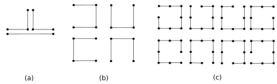
\includegraphics[width=12cm]{./img/b1epgSub.pdf}
\end{center}
\caption{Subfamílias Minimais não-Helly para $B_1$, $B_2$ e $B_3$ -families.}
\label{fig:b1b2b3families}
\end{figure}

Para $k=1$, seja $\cal{F}$ uma família de três caminhos de 1-dobra que são mutuamente intersectantes mas que não possuem aresta em comum, como ilustrado na Figura~\ref{fig:b1b2b3families}$(a)$. 
%For $k=1$, let $\cal{F}$ be the família %of three 1-dobra caminhos, $P_1: (0,0),(0,1),(1,1)$; $P_2: (1,1), (1,0),(0.2)$; and $P_3: (0,0),(0,2)$.  See Figure   $1a$. 
Então $\cal{F}$ é uma família de três caminhos  2-intersectante e $B_1$-EPG, tendo um core vazio. Portanto, $H(B_1$-EPG$) \geq 3$. 
Além disso, pela remoção de qualquer dos caminhos o core de $\cal{F}$ torna-se não-vazio. Todavia $\cal{F}$ é uma família de caminhos minimal não 2-Helly.

Seja $S$ o 4-ciclo, formado pelos 4 segmentos de pares de arestas, com dobras nos seguintes pontos da grade $(0,0),(0,2),(2,2),(2,0)$, respectivamente.
 Para $k= 2$,  considere $\cal{F}$ ser a família de quarto caminhos de 2-dobras formada quando removemos exatamente um par de arestas que formam os segmentos de cada lado do 4-ciclo, como ilustrado na  Figura~\ref{fig:b1b2b3families}$ (b)$.
Segue que $\cal{F}$ é 3-intersectante e seus caminhos não possuem nenhuma aresta comum. Consequentemente $H(B_2$-EPG)$ \geq 4$.

Para $k=3$, considere a família $\cal{F}$ de oito caminhos de  3-dobras, respectivamente, que podem ser obtidos de $S$. O 4-ciclo $S$ contem exatamente  8 arestas da grade. A  família $\cal{F}$ consiste de oito caminhos $P_i$, $1 \leq i \leq 8$, obtidos pela remoção de $S$, exatamente uma dessas oito arestas distintas, como ilustrado na Figura~\ref{fig:b1b2b3families} $ (c)$. Consequentemente, $\cal{F}$ é 7-intersectante, mas $core({\cal{F}}) = \emptyset$. Portanto, $H(B_3$-EPG)$\geq 8$.

Finalmente, para $k = 4$, seja $\cal{F}$ a família de $n$ $B_4$-caminhos $P_i$, descrita como segue:

\begin{itemize}
    \item $P_1$ é formado pelos segmentos: \\ $(0,0),(0,1),(1,1),(1,0),(n,0)$; 

     \item para $2 \leq i \leq n-1$, $P_i$ contem os segmentos: \\
     $(0,0),(0,i-1),(i-1,1),(i,1),(i,0),(n,0)$;
     
     \item  $P_n$ é formado pelos seguintes segmentos: \\ $(0,0),(n-1,0),(n-1,1),(n-1,0).$
     
\end{itemize}     

Observe que $\cal{F}$ é $(n-1)$-intersectante, enquanto $core({\cal{F}})=\emptyset$. Veja a Figura~\ref{fig:figurab4}. Dessa forma $H(B_4$-EPG) é ilimitado. Claramente o mesmo vale para $k >4$. \qed  



\begin{figure}[!h]
\begin{center}
% \begin{tikzpicture}[line cap=round,line join=round,>=triangle 45,x=3.7mm,y=3.7mm]
% \draw [color=cqcqcq,, xstep=0.74cm,ystep=0.74cm] (-7,-1.0) grid (22.8,14.8);
% \clip(-6.7,-1.8) rectangle (27,14.6);
% \draw [line width=2pt] (-6,0)-- (-6,2)-- (-4,2)-- (-4,0)-- (22,0);

% \draw [line width=2pt] (-6,4)-- (-4,4)-- (-4,6)-- (-2,6)-- (-2,4)-- (22,4);

% %\draw [line width=2pt] (-6,6)-- (-2,6)-- (-2,8)-- (0,8)-- (-0,6)-- (22,6);

% \draw [line width=2pt] (-6,8)-- (10,8)-- (10,10)-- (12,10)-- (12,8)-- (22,8);

% \draw [line width=2pt] (-6,12)-- (20,12)-- (20,14)-- (22,14)-- (22,12);


% \draw (6.5,6.5) node[anchor=north west] {.};
% \draw (6.5,7) node[anchor=north west] {.};
% \draw (6.5,7.5) node[anchor=north west] {.};

% \draw (6.5,10.5) node[anchor=north west] {.};
% \draw (6.5,11) node[anchor=north west] {.};
% \draw (6.5,11.5) node[anchor=north west] {.};

% \draw (-5.65,0.4) node[anchor=north west] {1};
% \draw (-3.65,3.4) node[anchor=north west] {2};

% %\draw (-1.65,6.4) node[anchor=north west] {3};

% \draw (10.35,8.4) node[anchor=north west] {i};

% \draw (20.35,12.4) node[anchor=north west] {n};

% \end{tikzpicture}
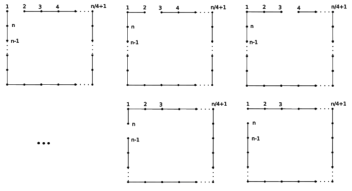
\includegraphics[width=12.5cm]{./img/b4epg.pdf}
\end{center}
\caption{$B_4$ possui número de Helly ilimitado.}\label{fig:figurab4}
\end{figure}

A seguir, nos preocupamos em encontrar limites superiores para grafos $H(B_k$-EPG).

\subsection{Limites Superiores}\label{subsec-upper}

De forma a obter um limite superior justo para o número de Helly, em termos do número de dobras, introduzimos abaixo mais algumas notações e lemas.

Dizemos que um conjunto de arestas da grade é {\it co-linear} se todas arestas do conjunto pertencem a uma mesma linha da grade, horizontal ou vertical. O conjunto de arestas é chamado {\it paralelo} se todas as suas arestas estiverem sobre linhas paralelas da grade mas nenhuma delas for co-linear.


\begin{lemma}
\label{lemma:3colin}
Seja $\cal {F}$ uma família minimal não-$(h-1)$-Helly de caminhos sobre uma grade contendo três arestas co-lineares não representativas. Então $\cal{F}$ deve conter caminhos com no mínimo quatro dobras.
\end{lemma}

\proof
Seja  $u_i$ a aresta do meio entre as três arestas  co-lineares não representativas. Ela corresponde ao caminho $P_i$ de $\cal {F'}$, não contendo $u_i$.
 Então $P_i$ deve passar pelas outras duas arestas mas ele não deve incluir a aresta do meio. Portanto, o caminho $P_i$ deve sair da linha comum da grade, contendo essas três arestas representativas, e retornar à mesma linha, assim requerendo no mínimo quatro dobras.
\qed


\begin{lemma}
\label{lemma:3par}
Seja $\cal{F}$ uma família minimal não-$(h-1)$-Helly de caminhos sobre uma grade, contendo três arestas paralelas, e tendo número de Helly $H(\cal{F})$   $\geq 4$. Então $\cal{F}$ deve conter caminhos com no mínimo quatro dobras. 
\end{lemma}

\proof
Uma vez que $H(\cal{F}) $ $\geq 4$ e $\cal{F}$ é uma $(h-1)$-família minimal, segue que $\cal{F}$ deve conter no mínimo quatro caminhos, $P_1,P_2,P_3,P_4$. Sem perda de generalidade, sejam $u_1,u_2,u_3$ as arestas não-representativas dos caminhos $P_1,P_2,P_3$ que são paralelas. Então $P_4$ deve passar por todas três arestas paralelas não-representativas $u_1,u_2,u_3$, assim requerendo no mínimo quatro dobras. 
\qed


\begin{lemma} \label{lemma:Lwit}
Seja $\cal{F}$ uma família minimal não-$(h-1)$-Helly de caminhos sobre uma grade com  número de Helly $H({\cal F}) \geq 4$. Se  ${\cal F}$ contem três arestas  não-representativas que se encontram sobre um mesmo $B_1$-caminho  $P_1$ de $\cal{F}$, então $\cal {F}$ deve possuir algum caminho com no mínimo três dobras. \end{lemma}

\proof
Visto que $\cal{F}$ é uma  $(h-1)$-família minimal tendo  número de Helly $\geq 4$, ela contem no mínimo quatro caminhos. Sem perda de generalidade, sejam  $u_1, u_2, u_3$ as três arestas não-representativas contidas em $P_4$ e tal que  $u_2$ encontra-se entre $u_1$ e $u_3$ em $P_4$. Então o caminho $P_2$ deve conter $u_1$ e $u_3$, mas evite $u_2$, assim requerendo no mínimo três dobras.  
\qed

A seguir são apresentados os limites superiores justos para os números de Helly de $B_k$-caminhos em arestas, para $k = 1,2,3$.

\begin{lema}\label{claim:upper-B1}
$H(B_1$-$EPG) \leq 3.$
\end{lema}
 
\proof
Assuma por contradição que o número de Helly de famílias de caminhos $B_1$-EPG é $h > 3$. Nesse caso, considere uma família minimal não-$(h-1)$-Helly $\cal F$ de caminhos $B_1$-EPG. Então $\cal F$ contem no mínimo  $h$ caminhos.  
Qualquer caminho $P_1 \in \cal{F}$ deve conter $h-1$ arestas não-representativas  correspondendo aos $h-1$ distintos caminhos de $\cal F$, diferentes de $P_i$. Uma vez que $h-1 \geq 3$, $P_1$  contem no mínimo três arestas  distintas não-representativas $u_2, u_3, u_4 \in P_1$, com $u_3$ encontrando-se entre $u_2$ e $u_4$ no caminho.  Se $P_1$ não possui dobras, $u_2,u_3,u_4$ são co-lineares. Pelo Lema~\ref{lemma:3colin},  o caminho $P_3 \in \cal{F}$ deve conter no mínimo quatro dobras. Se $P_1$ possui exatamente uma dobra, segue do Lema~\ref{lemma:Lwit} que $P_3$ possui três dobras. Em qualquer situação, uma contradição surge, implicando que $H({\cal F}) \leq 3$.
\qed

\begin{lema}\label{claim:upper-B2}
$H(B_2$-EPG$) \leq 4.$
\end{lema}

\proof
Assuma por contradição que o  número de Helly de famílias de caminhos  $B_2$-EPG é $h > 4$. Nesse caso, considere uma família minimal não-$(h-1)$-Helly  $\cal F$ de caminhos $B_2$-EPG. A família  $\cal F$ deve conter no mínimo $h \geq 5$ caminhos distintos, cada um deles correspondendo a uma aresta distinta  não-representativa. Selecione arbitrariamente 5 dessas arestas não-representativas.

Pelos Lemas~\ref{lemma:3colin} e ~\ref{lemma:3par} quaisquer dessas três arestas escolhidas não podem ser  co-lineares nem paralelas. Por consequência, no mínimo uma das 5 arestas não-representativas escolhidas deve estar em uma direção que é diferente da direção da maioria das outras arestas escolhidas. Chamemos a direção dessa aresta de vertical, e a direção da maioria das outras arestas de horizontal. Considere um caminho $P_1$ da família $\cal F$ que passa por essa aresta vertical. 
O caminho $P_1$ contem no mínimo quatro das arestas   não-representativas escolhidas, e no mínimo uma delas é vertical. Uma vez que $P_1$ possui no máximo duas dobras então ele deve ter no máximo três segmentos. Uma vez que temos três segmentos e quatro arestas não-representativas que $P_1$ deve conter, pelo princípio da casa dos pombos, um desses segmentos deve ter duas arestas não-representativas. Se esse par de arestas está em um segmento horizontal de $P_1$, então esse par de arestas, juntamente com a aresta vertical estão em dois segmentos consecutivos desse caminho, formando um $B_1$-subcaminho em $\cal F$. Então o Lema~\ref{lemma:Lwit} implica que algum caminho de $\cal F$ deve possuir no mínimo três dobras.  Caso contrário, as duas arestas seriam verticais. Mas as outras devem estar na  horizontal, e novamente temos no mínimo três arestas em um par de segmentos consecutivos formando um subcaminho em  $\cal F$ tendo uma dobra. Novamente, o  Lema ~\ref{lemma:Lwit} implica que algum caminho deve possuir no mínimo três dobras.
\qed

\begin{lema}\label{claim:upper-B3}
$H(B_3$-EPG$) \leq 8.$
\end{lema}

\proof
Assuma por contradição que o número de Helly de caminhos  $B_3$-EPG é $h > 8$. Nesse caso, considere uma família minimal não-$(h-1)$-Helly $\cal F$ de caminhos $B_3$-EPG. Então $\cal F$ contem no mínimo $h$  arestas não-representativas distintas,  correspondendo a  $h$ subconjuntos distintos. Pelo Lema~\ref{lemma:3par} já que podemos ter no máximo três dobras em qualquer caminho, então essas $h$ arestas  não-representativas devem encontrar-se em no máximo duas linhas vertical e horizontal da grade. Por esse motivo uma dessas quatro linhas possíveis deve conter pelo menos três arestas não-representativas distintas. Pelo  Lema~\ref{lemma:3colin},  isso implica na existência de um caminho com quatro dobras.\qed

Isso completa a prova do Teorema~\ref{thm:Helly-EPG}. 


\section{Número de Helly of $B_k$-VPG Graphs}\label{sec:helly-vpg}

Nessa seção determinaremos o número de Helly de grafos $B_k$-VPG. Para isso, provamos os seguintes resultados.
\begin{theorem}\label{thm:Bk-VPG}
O número de Helly para grafos $B_k$-VPG satisfaz:
\begin{enumerate}
\item $H(B_1$-VPG) = 4
\item $H(B_2$-VPG) = 6
\item $H(B_3$-VPG) = 12
\item $H(B_4$-VPG) é ilimitado.
\end{enumerate}
\end{theorem}

Novamente, a demonstração do teorema é efetuada pela apresentação de limites superiores e inferiores justos.

\subsection{Limites Inferiores}

Primeiro, apresentamos um conjunto de instâncias com caminhos que possuem no máximo $k$ dobras para delimitar um limite inferior para cada $k=1,2,3$.

A Figura~\ref{VPG:lower-B1} ilustra um conjunto de  quatro $B_1$-caminhos de um grafo $G$, em uma grade $2 \times 2$, tal que cada caminho cobre exatamente três vértices de  $G$, e evita exatamente um  dos  vértices. 

\begin{figure}[!h]
    \centering
    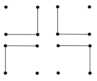
\includegraphics[width=3cm]{./img/lower-bound-B1-VPG.pdf}
    \caption{Limite inferior para grafos $B_1$-VPG.}
    \label{VPG:lower-B1}
\end{figure}

A Figura~\ref{VPG:lower-B2} ilustra um conjunto de seis $B_2$-caminhos de um grafo $G$, em uma grade  $2 \times 3$, tal que cada caminho cobre cinco vértices de $G$, e evita exatamente um.


\begin{figure}[!h]
    \centering
    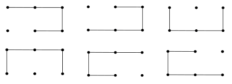
\includegraphics[width=8cm]{./img/lower-bound-B2-VPG.pdf}
    \caption{Limite inferior para grafos $B_2$-$VPG$.}
    \label{VPG:lower-B2}
\end{figure}


A Figura~\ref{VPG:lower-B3} ilustra um conjunto de doze $B_3$-caminhos de um grafo $G$, em uma grade, de perímetro 12, tal que cada caminho cobre  onze vértices de $G$, evitando um deles.

\begin{figure}[!h]
    \centering
    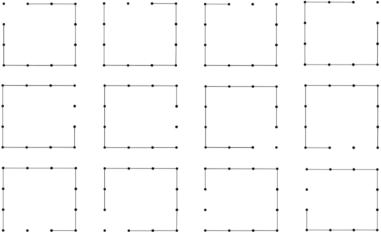
\includegraphics[width=12cm]{./img/lower-bound-B3-VPG.pdf}
    \caption{Limite inferior para grafos $B_3$-VPG.}
    \label{VPG:lower-B3}
\end{figure}

A Figura~\ref{VPG:lower-B4} ilustra um conjunto de $n$ $B_4$-caminhos de um grafo $G$ com $n$-vértices, em uma grade que possui perímetro $n$,  tal que cada caminho cobre exatamente   $n-1$  vértices do perímetro da grade, e evitando um deles. 

\begin{figure}[!h]
    \centering
    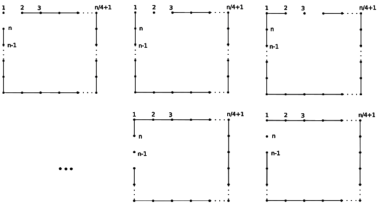
\includegraphics[width=12cm]{./img/lower-bound-B4-VPG.pdf}
    \caption{Limite inferior para grafos $B_4$-VPG.}
    \label{VPG:lower-B4}
\end{figure}

Aplicando o Teorema~\ref{thm:minimal}, podemos então concluir que o número de vértices de cada um dos grafos descritos anteriormente são limites inferiores para as classes correspondentes. Então, podemos estabelecer os seguintes limites.

\begin{lema}\label{claim:VPG-lower}
Os seguintes são limites inferiores para $H(B_k$-VPG).
\begin{enumerate}
\item $H(B_1$-VPG) $\geq 4$
\item $H(B_2$-VPG) $\geq 6$
\item $H(B_3$-VPG) $\geq 12$
\item $H(B_4$-VPG) é ilimitado.
\end{enumerate}
\end{lema}

\subsection{Limites Superiores}

A seguir, provamos limites superiores para o número de Helly de grafos $B_k$-VPG. Os seguintes lemas são empregados.

\begin{lemma}\label{column-sizes}
Seja $\cal F$ uma família minimal não-$(h-1)$-Helly de caminhos, para algum $h$, contendo $k \in \{3,4,5\}$ distintos pontos co-lineares não-representativos da grade. Então $\cal F$ contem um caminho com pelo menos $k-1$ dobras.
\end{lemma}

\proof Para $k \in \{3,5\}$, o caminho que evita o ponto do meio possui pelo menos $k-1$ dobras; enquanto para $k = 4$ o caminho evitando um dos pontos do meio também possui essa mesma propriedade.
\qed

\begin{lemma}\label{column-number}
Seja $\cal F$ uma família minimal não-$(h-1)$-Helly de caminhos, sobre uma grade contendo $k < h$ pontos distintos mutuamente não-co-lineares não-representativos. Então $\cal F$ deve conter um caminho com no mínimo $k-1$ dobras.
\end{lemma}   

\proof Uma vez que $k < h$, $\cal F$ deve conter um caminho que visite todos esses $k$ pontos mutuamente não-co-lineares. Esse caminho exige pelo menos uma dobra, entre dois pontos consecutivos não-co-lineares. Portanto $\cal F$ contem um caminho com pelo menos $k-1$ dobras. \qed \\

Também empregamos alguns conceitos e notações adicionais, descritos abaixo.

Seja $\cal F$ uma família minimal não-$(h-1)$-Helly  de $B_{k-1}$-caminhos sobre uma grade $Q$. Pelo Teorema~\ref{thm:minimal},  podemos escolher $h$ caminhos $P_i \in {\cal F}$, cada um deles associado a um ponto $p_i$ distinto não-representativo da grade, tal que $P_i$ evita $p_i$, mas contem todos os outros  $h-1$ pontos distintos não-representativos  $p_j \in P_J$, para cada $j \neq i$. Denote por $P_N$, $|P_N|=h$, o subconjunto de pontos da grade $Q$, restritos ao conjunto escolhido de distintos pontos  não-representativo $p_i$. Pelos Lemas~\ref{column-sizes} e \ref{column-number}, os pontos da grade de $P_N$ estão contidos em no máximo $k$ colunas (linhas), e cada  coluna (linha) contem no máximo $k$ pontos de $P_N$. Consequentemente, as cardinalidades dos pontos de $P_N$, contidas na coluna (linha) de $Q$,  forma uma partição  do inteiro $h$, em no máximo $k$ partes, tal que cada  parte possui tamanho no máximo  $k$. Chamemos tal partição como uma {\it partição viável de $h$, relativa a $P_N$}. Portanto, cada ponto não-representativo $p_i \in P_N$ contribui com uma unidade para alguma parte da partição, que é então referido como a parte da partição  {\it correspondendo} a $p_i$.    

O seguinte lema descreve condições suficientes para um inteiro $h$ ser um limite superior do número de Helly.

\begin{lemma}\label{upper-bound} Seja $\cal F$ uma família minimal não-$(h-1)$-Helly de $B_{k-1}$-caminhos sobre uma grade $Q$, e $P_N$ o conjunto de pontos não-representativos de $Q$. Sejam $k,h$ inteiros, $1 \leq k \leq 3$ e $k < h$. As seguintes condições implicam que $H(B_k$-VPG) $\leq h$  
\begin{itemize}
    \item[(i)] Não existe partição viável de $h+1$, relativa a $P_N$, ou 
    \item[(ii)] Para qualquer possível partição viável, e para qualquer disposição dos pontos da grade de $P_N$ em $Q$, existe algum ponto não-representativo  $p_i \in P_N$, tal que não existe caminho em $Q$, tendo no máximo  $k$ dobras, contendo todos pontos de $P_N$, exceto $p_i$.    
\end{itemize}
\end{lemma}
\proof A prova de (i) segue diretamente dos Lemas~\ref{column-sizes} e \ref{column-number}, enquanto a prova de (ii) é uma consequência do Teorema~\ref{thm:minimal}.  \qed \\

Os seguintes são limites superiores para o número de Helly de grafos $B_k$-VPG, para cada $k$, $1 \leq k \leq 3$, obtido pela aplicação do Lema~\ref{upper-bound}.      
 
\begin{lema}\label{claim:upper-B1-VPG}
$H(B_1$-VPG) $\leq  4$.
\end{lema}

\proof Não há partição do número inteiro 5, em 2 partes, em que cada parte possua no máximo 2 elementos. Consequentemente, o resultado segue do Lema~\ref{upper-bound}~(i). \qed

\begin{lema}\label{claim:upper-B2-VPG}
$H(B_2$-VPG)  $\leq  6$.
\end{lema}

\proof Assuma o contrário. Então $H(B_2$-VPG) $\geq  7$, seja $\cal F$ uma família minimal não-$6$-Helly de $B_2$-caminhos, e  $P_N$ seja o conjunto de pontos  não-representativos de $\cal F$ in $Q$. Existem duas partições viáveis do inteiro 7, em três partes, cada uma delas de tamanho no máximo 3, nomeadamente $(3,3,1)$ e $(3,2,2)$. Em qualquer desses casos  é sempre possível selecionar algum ponto $p_i \in P_N$, pertencendo a uma parte da partição de tamanho 3, tal que um caminho em  $\cal F$  que evite $p_i$ e cubra os outros  6 pontos não-representativos, deve conter pelo menos  3 dobras.  Então pelo Lema~\ref{upper-bound}, de fato $H(B_2$-VPG)  $\leq  6$. \qed


\begin{lema}\label{claim:upper-B3-VPG}
$H(B_3$-VPG) $\leq  12$.
\end{lema}

\proof Assuma por contradição que $H(B_3$-VPG) $\geq  12$. Seja $\cal F$ uma família minimal não-$12$-Helly de $B_3$-caminhos, e $P_N$ seja o conjunto de pontos não-representativos de $\cal F$ em $Q$. Existem três possíveis partições do inteiro 13, em quatro partes, tal que cada parte tenha tamanho máximo 4, nomeadamente $(4,4,4,1)$, $(4,4,3,2)$ e $(4,3,3,3)$. Nesse caso, selecione $p_i \in P_N$ para ser um ponto  não-representativo, correspondendo a uma parte de tamanho $4$ da partição.  O caminho de ${\cal F}$, que evita $p_i$ deve cobrir os outros 12 pontos não-representativos. Esses pontos estão localizados em 4 distintas colunas, de cardinalidades 4,4,3,1, 4,3,3,2, ou 3,3,3,3, considerando as 3 possíveis partições, respectivamente. Esse caminho deve conter no mínimo 4 dobras, uma contradição. Então pelo Lema~\ref{upper-bound}, $H(B_3$-VPG) $\leq  12$.    \qed  

Dos limites inferiores e superiores descritos nas subseções anteriores, obtemos os resultados para o  número de Helly de grafos $B_k$-VPG, completando a prova do Teorema~\ref{thm:Bk-VPG}.

\section{Número de Helly forte}\label{sec:helly-forte}

Nesta seção, consideramos uma maneira de determinar o número de Helly forte de grafos  $B_k$-EPG.

Iniciamos por descrever um teorema similar ao Teorema~\ref{thm:minimal}.

\begin{theorem}\label{thm:minimal-strong}

Seja ${\cal C}$ uma classe de famílias hereditárias  $\cal F$ de subconjuntos do conjunto universal $U$, cujo número de Helly forte  $sH({\cal C})$ é igual a $h$. Então existe uma família ${\cal F'} \in {\cal C}$ com exatamente $h$ subconjuntos satisfazendo a seguinte condição: 

Para cada subconjunto $P_i \in \cal {F'}$, há exatamente um elemento distinto $u_i \in U$, tal que 
$$u_i \not \in P_i,$$ 
mas $u_i$ está condido em todos subconjuntos 
$$P_j \in {\cal F'} \setminus P_i.$$
\end{theorem}

\proof O número de Helly forte  de ${\cal C}$ é $h$ e não $h - 1$, de modo que deva existir alguma família ${\cal F} \in {\cal C}$ cujo  número de Helly forte  é exatamente $h$, i.e. $\cal F$  contem $h$ subconjuntos $P_i$ cuja intersecção é igual ao core($\cal F'$) mas é tal que nenhum de seus  $h-1$ subconjuntos possui a mesma intersecção. Em particular, seja $\cal F'$ a família contendo exatamente os  $h$ subconjuntos $P_i$ descritos anteriormente. Essa  família deve existir, uma vez que $\cal C$ é hereditária. Então cada  $P_i$ não contem pelo menos um elemento $u_i$ na intersecção dos  $h-1$ subconjuntos restantes $P_j$, $j \ne i$, 
uma vez que a intersecção desses $h-1$ subconjuntos não deve ser igual ao core($\cal F'$).  \qed

Mais uma vez, se considerarmos a  família $\cal F'$ descrita no teorema anterior, então é simples concluir que a remoção de qualquer subconjunto de $\cal {F'}$ a torna $(h-1)$-Helly-forte.  Então denotamos $\cal {F'}$ como uma família {\it minimal} não-$(h-1)$-Helly-forte. Além disso, o elemento $u_i \not \in P_i$, contido em todos subconjuntos $P_j \in {\cal{F'}} \setminus P_i$, exceto $P_i$, é o {\it $h$ não-representativo} de $P_i$.  

Como antes, empregaremos os subconjuntos de famílias minimais já estabelecidos, aplicados a caminhos em uma grade.

De fato, provaremos que o número de Helly forte  de grafos $B_k$-EPG  coincide com o número de Helly, para cada valor de  $k$ correspondente. Similarmente, para grafos $B_k$-VPG. Para $k=0$, é  simples mostrar que se um conjunto de intervalos  $\cal I$ em uma linha mutuamente intersectam-se então existem dois intervalos de $\cal I$ cuja intersecção é igual à intersecção de todos os intervalos de $\cal I$. Consequentemente o $k$-número de Helly forte  de grafos $B_0$-EPG é igual a 2. 
Similarmente, o mesmo vale para grafos $B_0$-VPG. 
Relembrando que o número de Helly forte é pelo menos igual ao número de Helly de uma família, de modo que os limites inferiores apresentados  no Lema~\ref{claim:lower-Bk-EPG} também são válidos para o  número de Helly forte . As provas para o número de Helly forte s para $k \geq 1$ são similares às já descritas na Seção~\ref{sec:Helly-number}.  



\section{Considerações finais}\label{sec:finalRemarks4}

Nesse capítulo, determinamos o  número de Helly e o número de Helly forte  de grafos $B_k$-EPG e de grafos $B_k$-VPG, para $k \geq 0$. Os limites inferiores foram determinados pela apresentação de instâncias de conjuntos que definiam uma família de caminhos dentro de cada configuração. Por outro lado, os limites superiores foram determinados por abordagens matemáticas/geométricas que levaram em consideração fatos como as posições relativas de uma sequência de arestas (vértices) dos caminhos ou as possíveis subdivisões em partições de cada um de seus respectivos subconjuntos.

A Tabela \ref{tab:Helly-Strong-Helly} sumariza os resultados obtidos.
 
\Large 

\begin{table}[htb]
    \centering
    \begin{tabular}{c|c|c}
    \cline{1-3} $k$  & $B_k$-EPG & $B_k$-VPG \\
    \cline{1-3} 0 & 2 & 2 \\
    \cline{1-3} 1 & 3 & 4 \\
    \cline{1-3} 2 & 4 & 6 \\
    \cline{1-3} 3 & 8 & 12 \\
    \cline{1-3} $\geq 4$ & ilimitado & ilimitado \\
    \cline{1-3} 
    \end{tabular}
    \caption{Número de Helly e número de Helly forte para grafos $B_k$-EPG e $B_k$-VPG.}
    \label{tab:Helly-Strong-Helly}
\end{table}

\normalsize


Levantamos duas questões para serem investigadas, em relação aos resultados apresentados nesse capítulo.

\begin{enumerate}
\item Dado um {\it grafo específico}  EPG ou VPG, a  questão seria de formular um algoritmo capaz de determinar seu número de Helly e seu número de Helly forte. Ver o trabalho de~\cite{dourado2008improved}, para exemplos de tais algoritmos aplicados a grafos em geral.

\item Os valores do número de Helly e do número de Helly forte que foram determinados nesse capítulo coincidem em todos os casos. Claramente, em geral esse não é o caso. Deixamos uma questão em aberto, a de encontrar as condições para as quais essa igualdade ocorre.
\end{enumerate}


% \begin{thebibliography}{99}
% \bibitem{asinowski2011string}
% A. Asinowski, E. Cohen, M. C. Golumbic, V. Limouzy, M. Lipshteyn and M. Stern. Electronic Notes in Discrete Mathematics 37 (2011), pp. 141-146. 

% \bibitem{asinowski2012}  A. Asinowski, E. Cohen, M. C. Golumbic, V. Limouzy, M. Lipshteyn, and M. Stern,
% Vertex intersection graphs of caminhos on a grid, Journal of Graph Algorithms and
% Applications, 16 (2012) pp. 129-150.

% \bibitem{bergeDuchet1975}
% C. Berge and P. Duchet. A generalization of Gilmore’s theorem, {\emph in} M. Fiedler,
% editor, Recent Advances in Graph Theory, Acad. Praha, Prague, 1975, pp. 49-55

% \bibitem{duchet1978propriete}
% P. Duchet. Propriet\'e de Helly et probl\`emes de repr\'esentations. In Colloquium
% International CNRS 260, Probl\'emes Combinatoires et Th\'eorie de Graphs, Orsay, France, 1976, pp. 117-118

%  \bibitem{dourado2008improved}
%  M. C. Dourado, M. C. Lin, F. Protti, and J. L. Szwarcfiter. Improved algorithms
%  for recognizing $p$-Helly and hereditary $p$-Helly hypergraphs. Information Processing Letters 108  (2008), pp. 257-250.

% \bibitem{dourado2008strong}
% M. C. Dourado, F. Protti, and J. L. Szwarcfiter. On the strong $p$-Helly property.
% Discrete Applied Mathematics, 156 (2008), pp. 1053–1057

% \bibitem{dourado2009}
% M. C. Dourado, F. Protti and J. L. Szwarcfiter,
% Complexity aspects of the Helly
% property: graphs and hypergraphs. Electronic Journal on Combinatorics, Dynamic Surveys 17, 2009 

% \bibitem{golumbic1985}
% M. C. Golumbic and R. E. Jamison,
% The edge intersection graphs of caminhos in a tree,
% Journal of Combinatorial Theory B 38 (1985), pp. 8-22.

% \bibitem{golumbic2009}
% M. C. Golumbic, M. Lipshteyn and  M. Stern,
% Edge intersection graphs of single dobra caminhos on a grid, Networks 54 (2009), pp. 130-138.

% \bibitem{golumbic2013}
% M. C. Golumbic, M. Lipshteyn and  M. Stern,
% Single dobra caminhos on a grid have número de Helly forte  4,
% Networks (2013), 161-163

%\bibitem{}
% M. C. Golumbic and G. Morgenstern,
% Edge intersection graphs of caminhos
% on a grid, {\emph in} ``50 Years of Combinatorics, Graph Theory and Computing'', F.~Chung, R.~Graham, F.~Hoffman, L.~Hogben, R.~Mullin, D.~West, eds, CRC Press, 2019, pp. 193-209. 